% Options for packages loaded elsewhere
\PassOptionsToPackage{unicode}{hyperref}
\PassOptionsToPackage{hyphens}{url}
\PassOptionsToPackage{dvipsnames,svgnames,x11names}{xcolor}
%
\documentclass[
  letterpaper,
  numbers=noendperiod,
  fontsize=11pt,
  DIV=12,
  titlepage=false]{scrreprt}

\usepackage{amsmath,amssymb}
\usepackage{setspace}
\usepackage{iftex}
\ifPDFTeX
  \usepackage[T1]{fontenc}
  \usepackage[utf8]{inputenc}
  \usepackage{textcomp} % provide euro and other symbols
\else % if luatex or xetex
  \usepackage{unicode-math}
  \defaultfontfeatures{Scale=MatchLowercase}
  \defaultfontfeatures[\rmfamily]{Ligatures=TeX,Scale=1}
\fi
\usepackage{lmodern}
\ifPDFTeX\else  
    % xetex/luatex font selection
\fi
% Use upquote if available, for straight quotes in verbatim environments
\IfFileExists{upquote.sty}{\usepackage{upquote}}{}
\IfFileExists{microtype.sty}{% use microtype if available
  \usepackage[]{microtype}
  \UseMicrotypeSet[protrusion]{basicmath} % disable protrusion for tt fonts
}{}
\makeatletter
\@ifundefined{KOMAClassName}{% if non-KOMA class
  \IfFileExists{parskip.sty}{%
    \usepackage{parskip}
  }{% else
    \setlength{\parindent}{0pt}
    \setlength{\parskip}{6pt plus 2pt minus 1pt}}
}{% if KOMA class
  \KOMAoptions{parskip=half}}
\makeatother
\usepackage{xcolor}
\usepackage[top=30mm,bottom=30mm,left=25mm,right=25mm]{geometry}
\setlength{\emergencystretch}{3em} % prevent overfull lines
\setcounter{secnumdepth}{3}
% Make \paragraph and \subparagraph free-standing
\makeatletter
\ifx\paragraph\undefined\else
  \let\oldparagraph\paragraph
  \renewcommand{\paragraph}{
    \@ifstar
      \xxxParagraphStar
      \xxxParagraphNoStar
  }
  \newcommand{\xxxParagraphStar}[1]{\oldparagraph*{#1}\mbox{}}
  \newcommand{\xxxParagraphNoStar}[1]{\oldparagraph{#1}\mbox{}}
\fi
\ifx\subparagraph\undefined\else
  \let\oldsubparagraph\subparagraph
  \renewcommand{\subparagraph}{
    \@ifstar
      \xxxSubParagraphStar
      \xxxSubParagraphNoStar
  }
  \newcommand{\xxxSubParagraphStar}[1]{\oldsubparagraph*{#1}\mbox{}}
  \newcommand{\xxxSubParagraphNoStar}[1]{\oldsubparagraph{#1}\mbox{}}
\fi
\makeatother


\providecommand{\tightlist}{%
  \setlength{\itemsep}{0pt}\setlength{\parskip}{0pt}}\usepackage{longtable,booktabs,array}
\usepackage{calc} % for calculating minipage widths
% Correct order of tables after \paragraph or \subparagraph
\usepackage{etoolbox}
\makeatletter
\patchcmd\longtable{\par}{\if@noskipsec\mbox{}\fi\par}{}{}
\makeatother
% Allow footnotes in longtable head/foot
\IfFileExists{footnotehyper.sty}{\usepackage{footnotehyper}}{\usepackage{footnote}}
\makesavenoteenv{longtable}
\usepackage{graphicx}
\makeatletter
\def\maxwidth{\ifdim\Gin@nat@width>\linewidth\linewidth\else\Gin@nat@width\fi}
\def\maxheight{\ifdim\Gin@nat@height>\textheight\textheight\else\Gin@nat@height\fi}
\makeatother
% Scale images if necessary, so that they will not overflow the page
% margins by default, and it is still possible to overwrite the defaults
% using explicit options in \includegraphics[width, height, ...]{}
\setkeys{Gin}{width=\maxwidth,height=\maxheight,keepaspectratio}
% Set default figure placement to htbp
\makeatletter
\def\fps@figure{htbp}
\makeatother
% definitions for citeproc citations
\NewDocumentCommand\citeproctext{}{}
\NewDocumentCommand\citeproc{mm}{%
  \begingroup\def\citeproctext{#2}\cite{#1}\endgroup}
\makeatletter
 % allow citations to break across lines
 \let\@cite@ofmt\@firstofone
 % avoid brackets around text for \cite:
 \def\@biblabel#1{}
 \def\@cite#1#2{{#1\if@tempswa , #2\fi}}
\makeatother
\newlength{\cslhangindent}
\setlength{\cslhangindent}{1.5em}
\newlength{\csllabelwidth}
\setlength{\csllabelwidth}{3em}
\newenvironment{CSLReferences}[2] % #1 hanging-indent, #2 entry-spacing
 {\begin{list}{}{%
  \setlength{\itemindent}{0pt}
  \setlength{\leftmargin}{0pt}
  \setlength{\parsep}{0pt}
  % turn on hanging indent if param 1 is 1
  \ifodd #1
   \setlength{\leftmargin}{\cslhangindent}
   \setlength{\itemindent}{-1\cslhangindent}
  \fi
  % set entry spacing
  \setlength{\itemsep}{#2\baselineskip}}}
 {\end{list}}
\usepackage{calc}
\newcommand{\CSLBlock}[1]{\hfill\break\parbox[t]{\linewidth}{\strut\ignorespaces#1\strut}}
\newcommand{\CSLLeftMargin}[1]{\parbox[t]{\csllabelwidth}{\strut#1\strut}}
\newcommand{\CSLRightInline}[1]{\parbox[t]{\linewidth - \csllabelwidth}{\strut#1\strut}}
\newcommand{\CSLIndent}[1]{\hspace{\cslhangindent}#1}

\usepackage{booktabs}
\usepackage{longtable}
\usepackage{array}
\usepackage{float}
\usepackage{colortbl}
\usepackage{xcolor}
\usepackage{caption}
\usepackage{fancyhdr}
\captionsetup{font=small,labelfont=bf,skip=8pt}
\renewcommand{\arraystretch}{1.2}

% Configuración de encabezados
\pagestyle{fancy}
\fancyhf{}
\fancyhead[LE,RO]{\thepage}
\fancyhead[LO]{\nouppercase{\leftmark}}
\fancyhead[RE]{\nouppercase{\rightmark}}
\renewcommand{\headrulewidth}{0.4pt}

% Títulos de índices en español (después de babel/polyglossia)
\AtBeginDocument{%
  \renewcommand{\contentsname}{Índice General}%
  \renewcommand{\listfigurename}{Índice de Figuras}%
  \renewcommand{\listtablename}{Índice de Tablas}%
}
% Sin encabezado en páginas preliminares
\AtBeginDocument{
  \pagenumbering{roman}
  \pagestyle{plain}
}

% Configuración para numeración continua de capítulos (las partes no cuentan)
\makeatletter
% Ocultar numeración de partes
\renewcommand{\thepart}{}
% Remover el reset automático de capítulos por parte para numeración continua
\@removefromreset{chapter}{part}
% Hacer que las secciones se numeren basándose en el capítulo, no en la parte
\@removefromreset{section}{part}
% Asegurar que las secciones se numeren dentro de cada capítulo
\renewcommand{\thesection}{\thechapter.\arabic{section}}
\makeatother

% Configuración para evitar saltos de página innecesarios
\clubpenalty=10000
\widowpenalty=10000
\displaywidowpenalty=10000
\KOMAoption{captions}{tableheading}
\makeatletter
\@ifpackageloaded{bookmark}{}{\usepackage{bookmark}}
\makeatother
\makeatletter
\@ifpackageloaded{caption}{}{\usepackage{caption}}
\AtBeginDocument{%
\ifdefined\contentsname
  \renewcommand*\contentsname{Table of contents}
\else
  \newcommand\contentsname{Table of contents}
\fi
\ifdefined\listfigurename
  \renewcommand*\listfigurename{List of Figures}
\else
  \newcommand\listfigurename{List of Figures}
\fi
\ifdefined\listtablename
  \renewcommand*\listtablename{List of Tables}
\else
  \newcommand\listtablename{List of Tables}
\fi
\ifdefined\figurename
  \renewcommand*\figurename{Figure}
\else
  \newcommand\figurename{Figure}
\fi
\ifdefined\tablename
  \renewcommand*\tablename{Table}
\else
  \newcommand\tablename{Table}
\fi
}
\@ifpackageloaded{float}{}{\usepackage{float}}
\floatstyle{ruled}
\@ifundefined{c@chapter}{\newfloat{codelisting}{h}{lop}}{\newfloat{codelisting}{h}{lop}[chapter]}
\floatname{codelisting}{Listing}
\newcommand*\listoflistings{\listof{codelisting}{List of Listings}}
\makeatother
\makeatletter
\makeatother
\makeatletter
\@ifpackageloaded{caption}{}{\usepackage{caption}}
\@ifpackageloaded{subcaption}{}{\usepackage{subcaption}}
\makeatother

\ifLuaTeX
  \usepackage{selnolig}  % disable illegal ligatures
\fi
\usepackage{bookmark}

\IfFileExists{xurl.sty}{\usepackage{xurl}}{} % add URL line breaks if available
\urlstyle{same} % disable monospaced font for URLs
\hypersetup{
  colorlinks=true,
  linkcolor={NavyBlue},
  filecolor={Maroon},
  citecolor={NavyBlue},
  urlcolor={NavyBlue},
  pdfcreator={LaTeX via pandoc}}


\author{}
\date{}

\begin{document}

% ============================================================================
% PORTADA - PRIMERA PÁGINA DEL DOCUMENTO
% ============================================================================
\thispagestyle{empty}
\begin{center}

\vspace*{0.2cm}

% Logo

\includegraphics[width=0.20\textwidth]{logo/logo_udec.png}

\vspace{0.7cm}

% Título y Subtítulo
{\Huge\bfseries Derecha fragmentada y un enemigo compartido\par}
\vspace{0.4cm}
{\Large\itshape Análisis textual longitudinal de la constación discursiva en las elecciones presidencial de 2025 en Chile\par}

\vspace{0.9cm}

% Grado
{\large Tesis para optar al grado de\par}
\vspace{0.1cm}
{\large\bfseries Magíster en Ciencia de Datos\par}

\vspace{0.8cm}

% Autor
{\large\bfseries Matías Deneken\par}
\vspace{0.1cm}
{\normalsize Centro de Datos e Inteligencia Artificial - Universidad de Concepción\par}

\vspace{0.6cm}

% Profesores Guías
{\normalsize\bfseries Profesores Guías:\par}
\vspace{0.1cm}
{\normalsize Dr. Carlos Navarrete \par}
{\normalsize Dr. Marcela Parada \par}

\vspace{0.6cm}

% Universidad y Fecha
{\large Universidad de Concepción\par}
\vspace{0.2cm}
{\large Enero 2026\par}

\end{center}
\clearpage


\setstretch{1.5}
\bookmarksetup{startatroot}

\chapter*{Agradecimientos}\label{agradecimientos}
\addcontentsline{toc}{chapter}{Agradecimientos}

\markboth{Agradecimientos}{Agradecimientos}

Esta tesina no habría sido posible sin el apoyo económico de la beca de
excención de arancel por el Premio Universidad de Concepción, según
consta el decreto DIRPOST-021-24.

Agradezco a mis compañeras y compañeros de generación con los cuáles
compartí durante este proceso. En particular a Javiera Baeza y Florencia
Pampaloni, con quién constituí un excelente equipo de trabajo desde la
distancia. Sin este trabajo colaborativo la experiencia el MACI habría
sido significativamente más compleja.

De la misma forma, agradezco a nivel general mi experiencia en el MACI.
La pasantía realizada en la Universidad de Harvard en 2024 brindó una
oportunidad y riqueza iniguable para poder conocec un ecosistema que
-hasta entoces- me era ajeno. En particular, dar las gracias a mis
profesores guías, Marcela Parada y Carlos Navarrete, quiénes me
acompañaron en este proceso formativo.

Por último, darle siempre las gracias a mi familia por estimularla a
afrontar nuevas desafíos, incluso cuándo la energía es escasa.

Sin duda está tesis combina mis interéses de la sociología, a nivel de
pregrado y de magíster, y la ciencia de datos, que me ha conllevado a
esta incipiente área de las \emph{ciencias sociales computacionales}.
Con sus bemoles, espero que esta tesis sirva cómo mi puntapié inicial
para poder enfrentar nuevos desafíos que combine los métodos
estadísticos avanzado con la revolución de la Inteligencia Artificial
que hoy estamos viviendo. El tiempo nos dirá.

\newpage

\bookmarksetup{startatroot}

\chapter*{Presentación}\label{presentaciuxf3n}
\addcontentsline{toc}{chapter}{Presentación}

\markboth{Presentación}{Presentación}

Contenido de presentación/introducción general

\newpage

% Títulos de índices en español
\renewcommand{\contentsname}{Índice General}
\renewcommand{\listfigurename}{Índice de Figuras}
\renewcommand{\listtablename}{Índice de Tablas}
% Índices después de las páginas preliminares
\tableofcontents
\newpage
\listoffigures
\newpage
\listoftables
\newpage

% Cambiar a numeración arábiga para el contenido principal
\pagenumbering{arabic}
\pagestyle{fancy}

\bookmarksetup{startatroot}

\chapter{Introducción}\label{introducciuxf3n}

Las elecciones presidenciales chilenas de 2025 se desarrollan en un
contexto de profunda reconfiguración del sistema de partidos y de
transformación de las condiciones bajo las cuales se produce la
comunicación política. Tras el ciclo de movilizaciones iniciado en
octubre de 2019, los procesos constituyentes fallidos de 2022 y 2023, y
la creciente fragmentación de las coaliciones tradicionales, el
escenario electoral chileno exhibe niveles de incertidumbre, volatilidad
y polarización inéditos en la historia reciente del país.

En este contexto, las plataformas digitales han adquirido un
protagonismo sin precedentes como espacios de debate político, formación
de opinión y articulación de identidades colectivas. Lo que ocurre en
redes sociales ya no constituye un reflejo secundario de dinámicas
políticas que se dirimen en otros ámbitos, sino un terreno constitutivo
donde se disputan los términos del conflicto, se movilizan emociones
políticas y se construyen las fronteras simbólicas que delimitan aliados
y adversarios.

Una de las transformaciones más significativas del período reciente es
la reconfiguración del campo de las derechas chilenas. Donde antes
existía una coalición relativamente cohesionada ---heredera de la
transición democrática y articulada en torno a partidos como la UDI y
Renovación Nacional---, hoy convergen y compiten al menos tres
corrientes distinguibles: una derecha tradicional que busca renovar su
apelación desde la moderación y la competencia técnica; una derecha
radical-conservadora que articula posiciones morales restrictivas con
retórica antielitista; y una derecha libertaria de perfil disruptivo que
desafía las convenciones comunicativas establecidas. La competencia
entre estas corrientes, y su eventual convergencia frente a adversarios
comunes, constituye uno de los fenómenos más relevantes ---y menos
estudiados--- de la política chilena contemporánea.

\section{Justificación y relevancia del
estudio}\label{justificaciuxf3n-y-relevancia-del-estudio}

En la actualidad las encuestas, en general, y las de opinión, en
particular, han sido parte del escrutinio público. Este tipo de medición
han sido acusadas de fundar un datos sesgados y , en última instancia,
serviles a las tendencias ideológicas a las que se encuentran
posicionadas las que la financia o la consultora encargada.

Indepiente de esos juicios, las encuestas enfrentar problemas más allá.
El desafío principal es que las tasas de respuestas cada vez son más
bajas y los costos por la realización de la encuesta al individuo es
cada vez más caro. La era digital brindan oportunidades nuevas dado la
emergencia en del ``Big Data''. Es decir, la presencia de datos masivos.

Esta investigación se justifica en función de tres órdenes de
consideraciones: empíricas, teóricas y metodológicas.

Desde el punto de vista \textbf{empírico}, el ciclo electoral chileno de
2025 ofrece una oportunidad única para observar en tiempo real las
dinámicas de competencia intra-derecha en un sistema político en
transformación. La coexistencia de tres candidaturas de derecha con
perfiles ideológicos y estrategias comunicativas diferenciadas ---Evelyn
Matthei, José Antonio Kast y Johannes Kaiser--- permite analizar
comparativamente cómo distintas corrientes construyen sus identidades,
movilizan usuarios y se posicionan frente a adversarios internos y
externos. La presencia de una candidatura de izquierda asociada al
Partido Comunista ---Jeannette Jara--- añade una dimensión adicional al
análisis, habilitando el estudio de los procesos de convergencia
discursiva que emergen cuando actores previamente enfrentados deben
articular un frente común.

Desde el punto de vista \textbf{teórico}, la investigación contribuye a
debates contemporáneos sobre comunicación política digital, polarización
y construcción de antagonismos. Si bien existe abundante literatura
sobre el rol de las redes sociales en procesos electorales, la mayor
parte de esta investigación se ha concentrado en contextos del Norte
Global, particularmente Estados Unidos y Europa Occidental. Los estudios
sobre América Latina, aunque crecientes, han tendido a focalizarse en
casos de alta visibilidad internacional ---Brasil con Bolsonaro,
Argentina con Milei--- sin atender suficientemente a las variaciones
nacionales y a las dinámicas de competencia al interior de familias
ideológicas. Esta tesis busca contribuir a llenar ese vacío, ofreciendo
un análisis detallado de las especificidades del caso chileno.

Desde el punto de vista \textbf{metodológico}, la investigación propone
una aproximación que integra técnicas de ciencia social computacional
con análisis interpretativo del discurso político. Esta combinación
permite procesar volúmenes de datos que excederían las capacidades del
análisis cualitativo tradicional, sin sacrificar la atención a las
dimensiones semánticas y pragmáticas que resultan cruciales para
comprender la comunicación política. La elección de Reddit como campo de
observación ---una plataforma subexplorada en el contexto
latinoamericano--- ofrece además la posibilidad de acceder a
conversaciones políticas con características estructurales distintivas
que enriquecen el análisis.

\section{Preguntas de
investigación}\label{preguntas-de-investigaciuxf3n}

La pregunta central que orienta esta investigación es:

\begin{quote}
\textbf{¿Cómo se configura y evoluciona la conversación política en
Reddit durante la campaña presidencial chilena de 2025?}
\end{quote}

Esta pregunta general se desagrega en las siguientes interrogantes
específicas:

\begin{enumerate}
\def\labelenumi{\arabic{enumi}.}
\item
  ¿Qué patrones de encuadre (\emph{framing}), movilización emocional y
  construcción de adversarios estructuran el debate político en los
  subreddits chilenos durante el período electoral?
\item
  ¿Cómo varían temporalmente las estrategias discursivas de ataque,
  defensa y demarcación de fronteras identitarias a lo largo de las
  distintas fases de la campaña?
\item
  ¿Qué dinámicas de competencia, diferenciación y antagonismo se
  observan entre las tres corrientes de derecha (tradicional,
  radical-conservadora y libertaria) durante la primera vuelta?
\item
  ¿Cómo se produce la convergencia discursiva en torno al Partido
  Comunista como adversario común durante la segunda vuelta, y qué
  tensiones persisten bajo esta convergencia aparente?
\end{enumerate}

\section{Objetivos de la
investigación}\label{objetivos-de-la-investigaciuxf3n}

\subsection{Objetivo general}\label{objetivo-general}

Analizar la configuración y evolución de la conversación política en
Reddit durante la campaña presidencial chilena de 2025, identificando
los patrones de encuadre, emoción y construcción de adversarios que
estructuran el debate entre las distintas corrientes ideológicas.

\subsection{Objetivos específicos}\label{objetivos-especuxedficos}

\begin{enumerate}
\def\labelenumi{\arabic{enumi}.}
\item
  Caracterizar los marcos interpretativos (\emph{frames}) predominantes
  en el discurso de cada corriente ideológica y su variación a lo largo
  del ciclo electoral.
\item
  Identificar los patrones de movilización emocional asociados a cada
  candidatura, distinguiendo emociones de valencia positiva, negativa y
  las combinaciones que configuran repertorios afectivos específicos
\item
  Analizar las estrategias de construcción de adversarios, atendiendo
  tanto a la definición de enemigos externos (inter-bloque) como a las
  dinámicas de diferenciación interna (intra-bloque).
\item
  Examinar la evolución temporal del debate, identificando puntos de
  inflexión, eventos catalizadores y patrones de activación discursiva
  asociados a momentos específicos de la campaña.
\end{enumerate}

\bookmarksetup{startatroot}

\chapter{Presentación del Problema}\label{presentaciuxf3n-del-problema}

\section{El problema: competencia política digital en un sistema
fragmentado}\label{el-problema-competencia-poluxedtica-digital-en-un-sistema-fragmentado}

El sistema de partidos chileno atraviesa una crisis de representación
sin precedentes desde el retorno a la democracia. Los indicadores son
contundentes: la identificación partidaria ha caído sostenidamente desde
2010, la volatilidad electoral alcanzó máximos históricos en los ciclos
2021-2023, y la fragmentación parlamentaria dificulta la formación de
coaliciones estables (PNUD, 2024; Luna, 2023). En este contexto de
desalineamiento, las plataformas digitales han emergido como espacios
donde se disputa la reconfiguración de las identidades políticas
---particularmente en el campo de las derechas, donde coexisten
proyectos en competencia que aún no han estabilizado sus fronteras.

El \textbf{problema central} que aborda esta investigación puede
formularse así:

\begin{quote}
En un contexto de fragmentación partidaria y reconfiguración ideológica,
¿cómo se estructura la competencia política digital entre actores que
comparten un espacio ideológico pero compiten por diferenciarse? ¿Qué
estrategias discursivas despliegan? ¿Bajo qué condiciones convergen o
divergen?
\end{quote}

Este problema es relevante por tres razones:

\begin{enumerate}
\def\labelenumi{\arabic{enumi}.}
\item
  \textbf{Vacío empírico}: Mientras abundan los estudios sobre
  polarización izquierda-derecha, la competencia \emph{intra-bloque}
  ---particularmente entre derechas--- permanece subexplorada en América
  Latina.
\item
  \textbf{Transformación en curso}: Las derechas chilenas están en
  proceso de reconfiguración activa; estudiar este proceso mientras
  ocurre permite capturar dinámicas que análisis retrospectivos pierden.
\item
  \textbf{Implicancias democráticas}: Comprender cómo se construyen
  adversarios y fronteras identitarias en espacios digitales resulta
  crucial para evaluar la calidad del debate público y anticipar
  escenarios de polarización.
\end{enumerate}

\section{Acercamiento: actores, dimensiones y niveles de
análisis}\label{acercamiento-actores-dimensiones-y-niveles-de-anuxe1lisis}

\subsection{Los actores: tres derechas y un
adversario}\label{los-actores-tres-derechas-y-un-adversario}

La investigación se focaliza en cuatro candidaturas que representan
posiciones distintivas en el espectro político chileno:

\begin{longtable}[]{@{}
  >{\raggedright\arraybackslash}p{(\columnwidth - 6\tabcolsep) * \real{0.2113}}
  >{\raggedright\arraybackslash}p{(\columnwidth - 6\tabcolsep) * \real{0.2113}}
  >{\raggedright\arraybackslash}p{(\columnwidth - 6\tabcolsep) * \real{0.3662}}
  >{\raggedright\arraybackslash}p{(\columnwidth - 6\tabcolsep) * \real{0.2113}}@{}}
\caption{Candidaturas incluidas en el análisis y su caracterización
ideológica. }\label{tbl-candidaturas-actores}\tabularnewline
\toprule\noalign{}
\begin{minipage}[b]{\linewidth}\raggedright
Actor
\end{minipage} & \begin{minipage}[b]{\linewidth}\raggedright
Posición
\end{minipage} & \begin{minipage}[b]{\linewidth}\raggedright
Caracterización sintética
\end{minipage} & \begin{minipage}[b]{\linewidth}\raggedright
Base social
\end{minipage} \\
\midrule\noalign{}
\endfirsthead
\toprule\noalign{}
\begin{minipage}[b]{\linewidth}\raggedright
Actor
\end{minipage} & \begin{minipage}[b]{\linewidth}\raggedright
Posición
\end{minipage} & \begin{minipage}[b]{\linewidth}\raggedright
Caracterización sintética
\end{minipage} & \begin{minipage}[b]{\linewidth}\raggedright
Base social
\end{minipage} \\
\midrule\noalign{}
\endhead
\bottomrule\noalign{}
\endlastfoot
\textbf{Evelyn Matthei} & Derecha tradicional & Pragmatismo, competencia
técnica, moderación discursiva & Élites empresariales, sectores
medios-altos \\
\textbf{José Antonio Kast} & Derecha radical-conservadora &
Conservadurismo moral, retórica antielitista, énfasis en seguridad y
migración & Sectores populares conservadores, evangélicos \\
\textbf{Johannes Kaiser} & Derecha libertaria & Ultraliberalismo,
provocación deliberada, códigos de subculturas digitales & Jóvenes
masculinos, usuarios intensivos de internet \\
\textbf{Jeannette Jara} & Izquierda-PC & Proyecto transformador, defensa
del legado del gobierno Boric & Militancia de izquierda, sectores
sindicalizados \\
\end{longtable}

Como se observa en la Table~\ref{tbl-candidaturas-actores}, el diseño
compara tres derechas y un adversario común de izquierda.

Esta selección permite observar:

\begin{itemize}
\tightlist
\item
  \textbf{Competencia intra-derecha}: Cómo tres proyectos distintos
  disputan un electorado parcialmente superpuesto.
\item
  \textbf{Convergencia anti-izquierda}: Cómo actores previamente
  enfrentados articulan un frente común frente al adversario ideológico.
\item
  \textbf{Asimetrías discursivas}: Cómo diferentes corrientes movilizan
  repertorios retóricos y emocionales distintivos.
\end{itemize}

\subsection{Las dimensiones
analíticas}\label{las-dimensiones-analuxedticas}

El análisis se estructura en torno a \textbf{tres dimensiones} que
capturan aspectos complementarios de la comunicación política:

\textbf{Dimensión 1: Encuadre (\emph{framing})} - ¿Qué marcos
interpretativos predominan en el discurso de cada corriente? - ¿Cómo
definen el problema, sus causas y sus soluciones? - ¿Qué está ``en
juego'' según cada actor?

\textbf{Dimensión 2: Emoción} - ¿Qué emociones movilizan las distintas
candidaturas? - ¿Cuál es la proporción entre emociones positivas
(entusiasmo, esperanza) y negativas (miedo, indignación)? - ¿Hacia quién
se dirigen las emociones negativas?

\textbf{Dimensión 3: Construcción de adversarios} - ¿Quiénes son
construidos como amenazas o enemigos? - ¿Qué estrategias de
deslegitimación se emplean? - ¿Cómo se articulan los antagonismos
inter-bloque (derecha vs. izquierda) con los intra-bloque (entre
derechas)?

\subsection{Los niveles de análisis}\label{los-niveles-de-anuxe1lisis}

El diseño contempla tres niveles de observación:

\begin{longtable}[]{@{}
  >{\raggedright\arraybackslash}p{(\columnwidth - 4\tabcolsep) * \real{0.2500}}
  >{\raggedright\arraybackslash}p{(\columnwidth - 4\tabcolsep) * \real{0.2639}}
  >{\raggedright\arraybackslash}p{(\columnwidth - 4\tabcolsep) * \real{0.4861}}@{}}
\caption{Niveles de análisis utilizados en la investigación.
}\label{tbl-niveles-analisis}\tabularnewline
\toprule\noalign{}
\begin{minipage}[b]{\linewidth}\raggedright
Nivel
\end{minipage} & \begin{minipage}[b]{\linewidth}\raggedright
Unidad
\end{minipage} & \begin{minipage}[b]{\linewidth}\raggedright
Foco analítico
\end{minipage} \\
\midrule\noalign{}
\endfirsthead
\toprule\noalign{}
\begin{minipage}[b]{\linewidth}\raggedright
Nivel
\end{minipage} & \begin{minipage}[b]{\linewidth}\raggedright
Unidad
\end{minipage} & \begin{minipage}[b]{\linewidth}\raggedright
Foco analítico
\end{minipage} \\
\midrule\noalign{}
\endhead
\bottomrule\noalign{}
\endlastfoot
\textbf{Macro} & Corpus completo & Tendencias agregadas, evolución
temporal, comparación entre subreddits \\
\textbf{Meso} & Hilos de discusión & Dinámicas conversacionales,
patrones de confrontación/consenso \\
\textbf{Micro} & Posts y comentarios individuales & Estrategias
retóricas específicas, ejemplos ilustrativos \\
\end{longtable}

La Table~\ref{tbl-niveles-analisis} resume cómo se articula el análisis
en escalas macro, meso y micro.

\section{Descripción de la propuesta
analítica}\label{descripciuxf3n-de-la-propuesta-analuxedtica}

\subsection{Enfoque general}\label{enfoque-general}

La propuesta combina \textbf{ciencia social computacional} con
\textbf{análisis interpretativo del discurso político}. Esta combinación
responde a una convicción metodológica: las técnicas computacionales
permiten identificar patrones a escala que el análisis cualitativo
tradicional no alcanza, pero requieren interpretación teóricamente
informada para producir conocimiento sustantivo sobre procesos
políticos.

El flujo analítico puede representarse así:

\begin{figure}[H]

{\centering 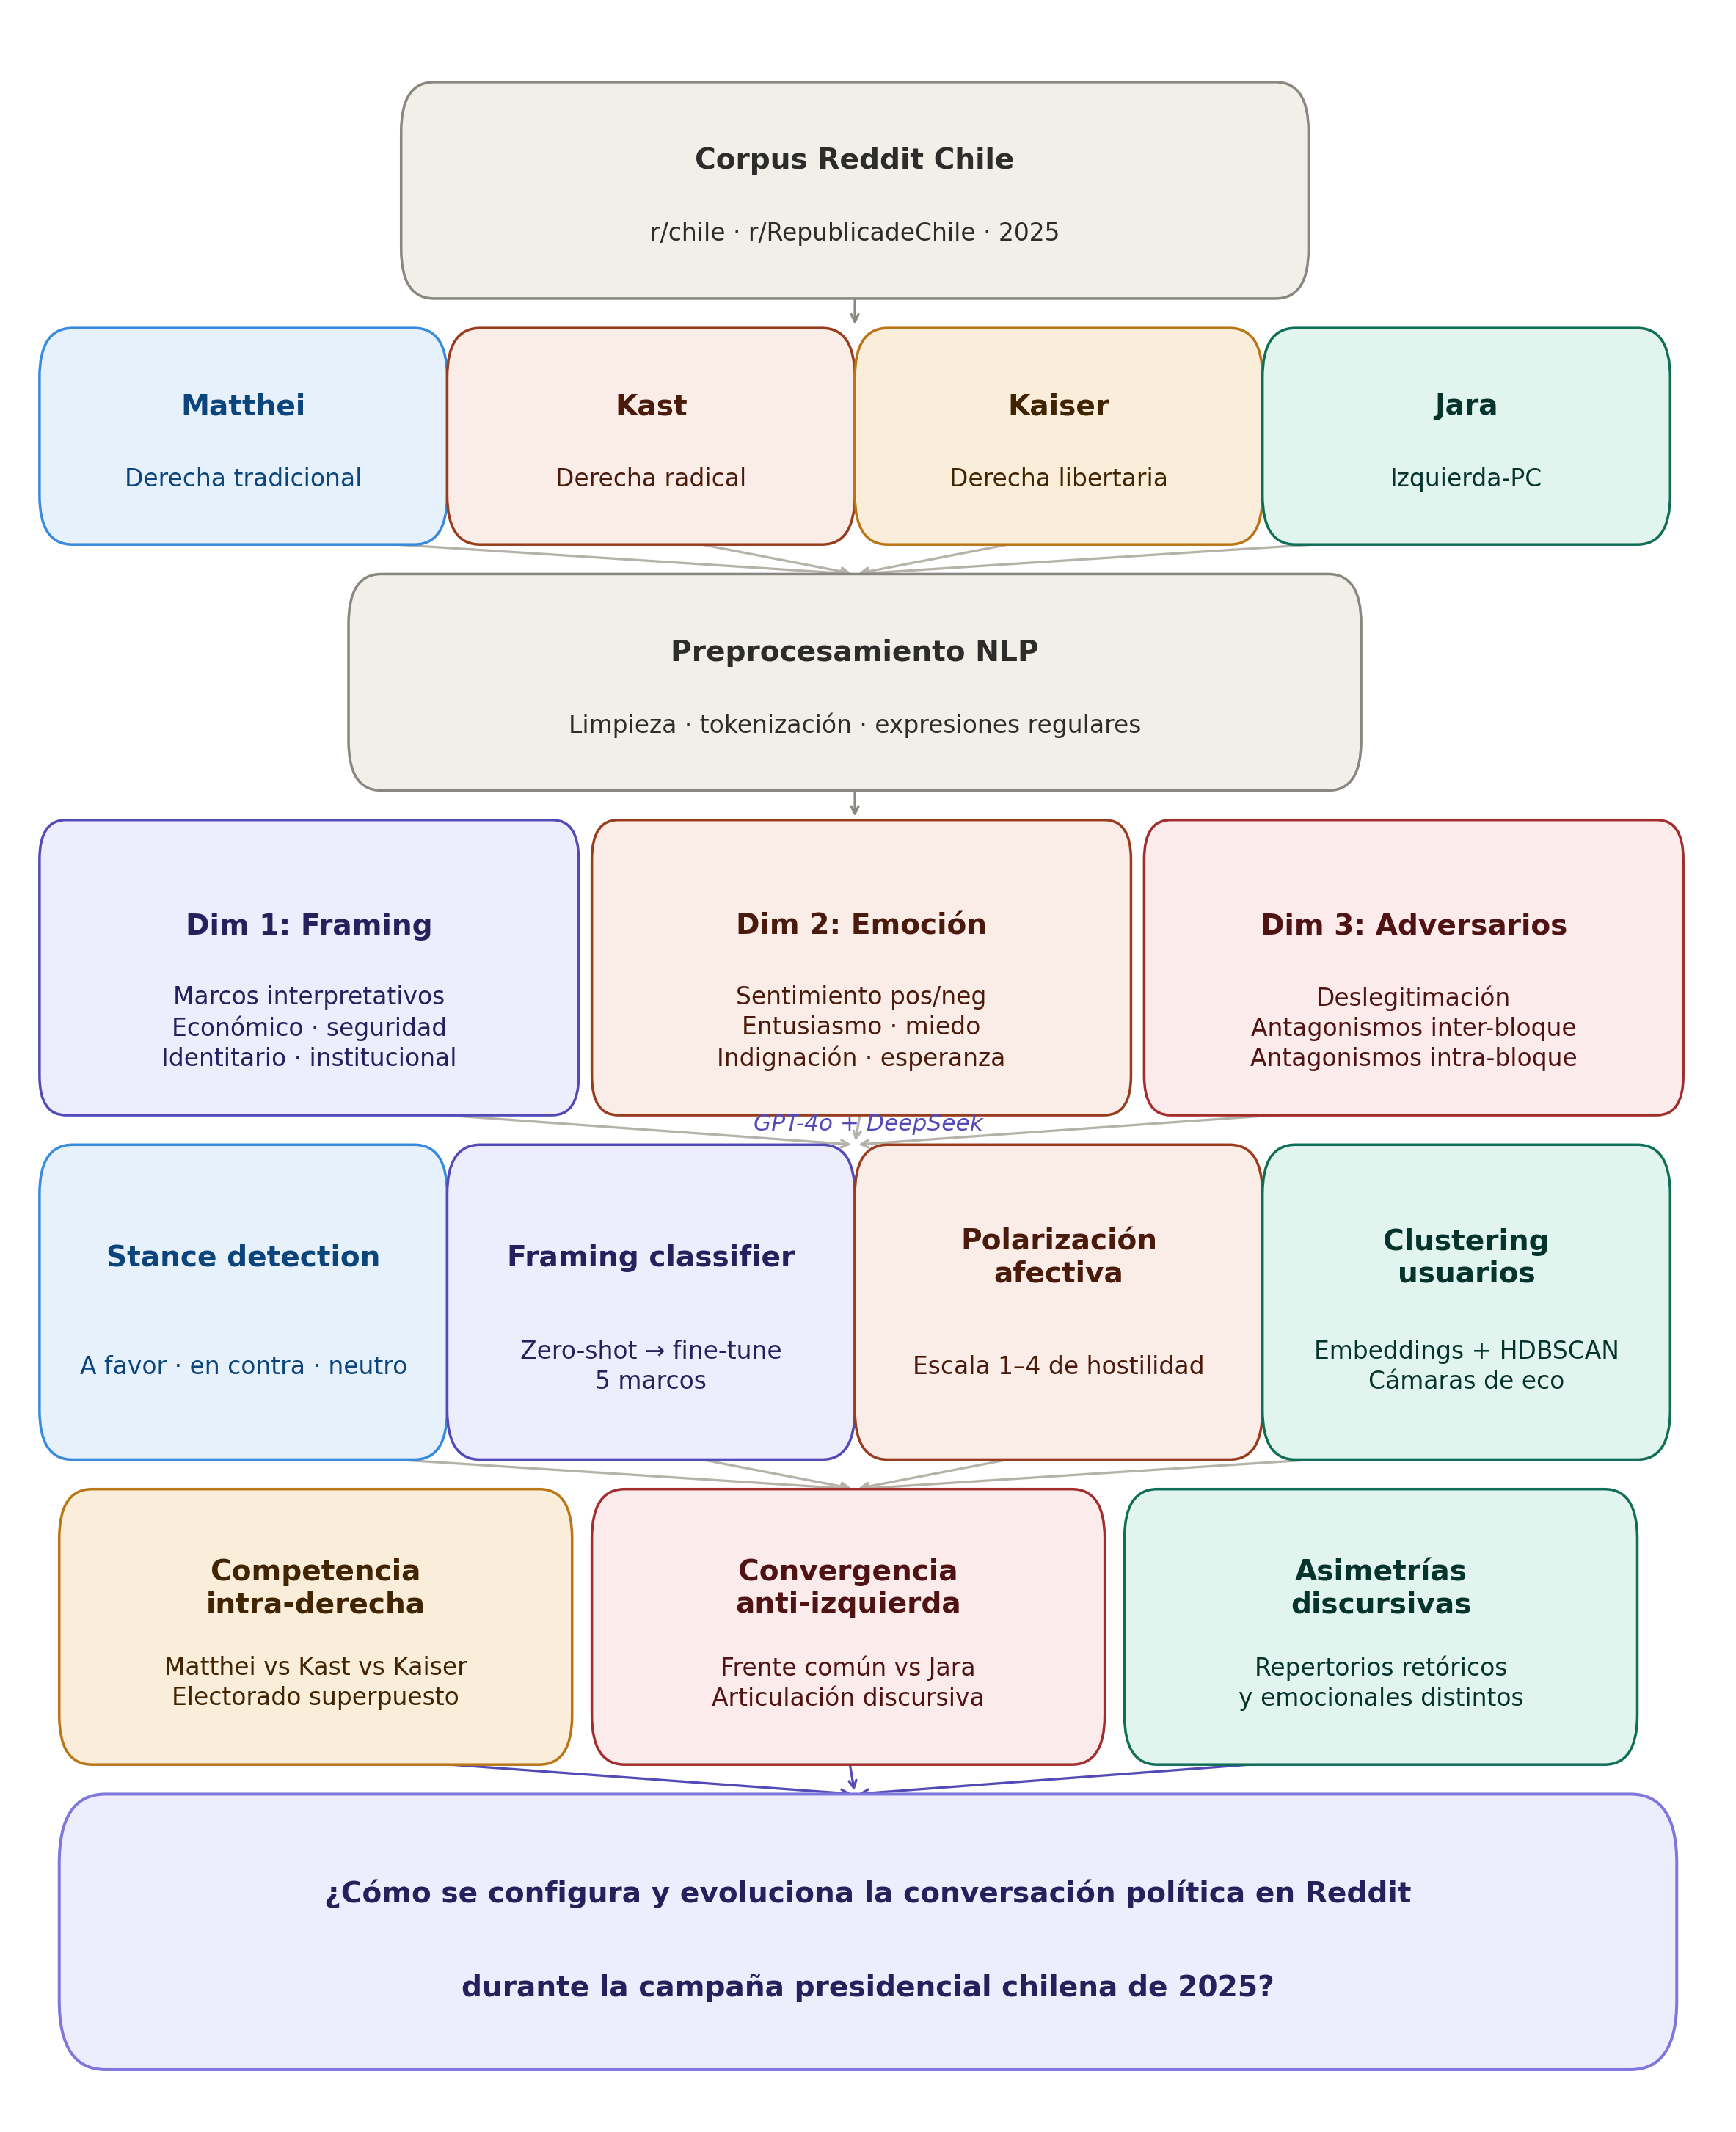
\includegraphics[width=0.75\textwidth,height=\textheight]{images/diagrama.png}

}

\caption{Pipeline analítico: de la recolección del corpus a los
hallazgos sustantivos.}

\end{figure}%

La \textbf{?@fig-pipeline} sintetiza el encadenamiento entre corpus,
procesamiento, modelamiento y hallazgos.

\subsection{Arquitectura del
análisis}\label{arquitectura-del-anuxe1lisis}

\textbf{Fase 1: Caracterización del corpus} - Estadísticas descriptivas:
volumen, distribución temporal, participación por subreddit - Mapeo de
actores: frecuencia de mención de cada candidatura - Identificación de
eventos: picos de actividad y su correlación con acontecimientos
políticos

\textbf{Fase 2: Análisis de encuadres} - Modelado de tópicos para
identificar temas estructurantes - Análisis de co-ocurrencias: qué
conceptos aparecen asociados a cada candidatura - Comparación
inter-temporal: evolución de marcos entre primera y segunda vuelta

\textbf{Fase 3: Análisis emocional} - Clasificación de sentimiento
(positivo/negativo/neutro) - Identificación de emociones discretas
cuando es posible - Construcción de ``perfiles emocionales'' por
candidatura

\textbf{Fase 4: Análisis de adversarios} - Identificación de menciones
cruzadas entre candidaturas - Clasificación de valencia: menciones
positivas, negativas, neutras - Mapeo de redes de antagonismo

\textbf{Fase 5: Síntesis e integración} - Triangulación de hallazgos
entre dimensiones - Construcción de narrativa analítica - Identificación
de mecanismos explicativos

\subsection{Originalidad de la
propuesta}\label{originalidad-de-la-propuesta}

La propuesta se distingue de estudios previos en tres aspectos:

\begin{enumerate}
\def\labelenumi{\arabic{enumi}.}
\item
  \textbf{Foco en competencia intra-bloque}: Mientras la mayoría de
  estudios examina la polarización entre izquierda y derecha, esta
  investigación centra la atención en las dinámicas \emph{dentro} del
  campo de las derechas.
\item
  \textbf{Perspectiva procesual}: En lugar de fotografías estáticas, el
  diseño longitudinal permite observar cómo evolucionan las estrategias
  discursivas a lo largo del ciclo electoral.
\item
  \textbf{Reddit como campo}: La plataforma está subexplorada en el
  contexto latinoamericano, y sus características estructurales
  (conversaciones anidadas, votación comunitaria) ofrecen posibilidades
  analíticas distintivas.
\end{enumerate}

\section{Producto mínimo viable (MVP) y objetivos
operacionales}\label{producto-muxednimo-viable-mvp-y-objetivos-operacionales}

\subsection{Definición del MVP}\label{definiciuxf3n-del-mvp}

El \textbf{producto mínimo viable} de esta investigación consiste en:

\begin{quote}
Un análisis sistemático de la conversación política en Reddit sobre las
candidaturas presidenciales chilenas de 2025, que identifique y
caracterice los patrones de encuadre, emoción y construcción de
adversarios de cada corriente ideológica, y que documente su evolución a
lo largo del ciclo electoral (agosto-diciembre 2024).
\end{quote}

\subsection{Objetivos operacionales y
entregables}\label{objetivos-operacionales-y-entregables}

\begin{longtable}[]{@{}
  >{\raggedright\arraybackslash}p{(\columnwidth - 4\tabcolsep) * \real{0.2466}}
  >{\raggedright\arraybackslash}p{(\columnwidth - 4\tabcolsep) * \real{0.2466}}
  >{\raggedright\arraybackslash}p{(\columnwidth - 4\tabcolsep) * \real{0.5068}}@{}}
\caption{Objetivos operacionales, entregables e indicadores de
cumplimiento del MVP.}\label{tbl-objetivos-mvp}\tabularnewline
\toprule\noalign{}
\begin{minipage}[b]{\linewidth}\raggedright
Objetivo
\end{minipage} & \begin{minipage}[b]{\linewidth}\raggedright
Entregable
\end{minipage} & \begin{minipage}[b]{\linewidth}\raggedright
Indicador de cumplimiento
\end{minipage} \\
\midrule\noalign{}
\endfirsthead
\toprule\noalign{}
\begin{minipage}[b]{\linewidth}\raggedright
Objetivo
\end{minipage} & \begin{minipage}[b]{\linewidth}\raggedright
Entregable
\end{minipage} & \begin{minipage}[b]{\linewidth}\raggedright
Indicador de cumplimiento
\end{minipage} \\
\midrule\noalign{}
\endhead
\bottomrule\noalign{}
\endlastfoot
\textbf{O1}: Construir corpus & Base de datos estructurada & ≥1000 posts
y ≥10.000 comentarios con menciones políticas \\
\textbf{O2}: Caracterizar encuadres & Modelo de tópicos interpretado &
Identificación de ≥5 marcos distintivos por corriente \\
\textbf{O3}: Mapear emociones & Perfiles emocionales por candidatura &
Clasificación de sentimiento del 100\% del corpus \\
\textbf{O4}: Analizar adversarios & Red de antagonismos & Matriz de
menciones cruzadas con valencia \\
\textbf{O5}: Documentar evolución & Serie temporal & Análisis por fase
electoral (pre-campaña, campaña, segunda vuelta) \\
\textbf{O6}: Sintetizar hallazgos & Capítulos de resultados & Respuesta
fundamentada a cada pregunta de investigación \\
\end{longtable}

La planificación operativa del estudio se detalla en la
Table~\ref{tbl-objetivos-mvp}.

\subsection{Alcances y limitaciones
anticipadas}\label{alcances-y-limitaciones-anticipadas}

\textbf{Alcances}: - El análisis cubre el debate en dos comunidades de
Reddit, que constituyen los principales espacios de discusión política
chilena en la plataforma. - El período captura fases clave del ciclo
electoral, permitiendo observar dinámicas de cambio. - Las técnicas
empleadas permiten procesar el corpus completo, no solo muestras.

\textbf{Limitaciones}: - Reddit no es representativo del electorado
chileno; los hallazgos refieren al debate en esta plataforma específica,
no a la opinión pública general. - Los usuarios de Reddit tienden a ser
más jóvenes, más masculinos y más politizados que la población general.
- El análisis de sentimiento automatizado tiene márgenes de error,
particularmente con ironía, sarcasmo y jerga local. - La atribución
ideológica de usuarios es inferida a partir de su comportamiento
discursivo, no de autodeclaraciones.

\section{Estrategia de validación}\label{estrategia-de-validaciuxf3n}

\subsection{Validación interna}\label{validaciuxf3n-interna}

\textbf{Triangulación metodológica}: Los hallazgos de cada técnica
(modelado de tópicos, análisis de sentimiento, análisis de redes) son
contrastados entre sí. Un patrón se considera robusto cuando emerge
consistentemente de múltiples aproximaciones.

\textbf{Verificación cualitativa}: Los patrones identificados
computacionalmente son verificados mediante lectura de casos. Cuando el
análisis automatizado clasifica un comentario como ``negativo hacia
Matthei'', se revisan ejemplos para confirmar que la clasificación
captura el fenómeno de interés.

\textbf{Sensibilidad paramétrica}: Las técnicas con parámetros
ajustables (número de tópicos, umbrales de clasificación) son ejecutadas
con múltiples configuraciones para verificar que los hallazgos no
dependan de decisiones arbitrarias.

\subsection{Validación externa}\label{validaciuxf3n-externa}

\textbf{Triangulación con fuentes externas}: Los patrones temporales
identificados en Reddit son contrastados con el calendario de eventos
políticos documentado en medios de comunicación. La correlación entre
picos de actividad y eventos específicos (debates, declaraciones,
encuestas) proporciona validación externa.

\textbf{Consistencia con literatura}: Los hallazgos son discutidos a la
luz de estudios previos sobre comunicación política digital, derechas
latinoamericanas y polarización. La convergencia con patrones
documentados en otros contextos refuerza la validez; las divergencias
son examinadas como posibles especificidades del caso chileno.

\subsection{Criterios de éxito}\label{criterios-de-uxe9xito}

La investigación se considerará exitosa si:

\begin{enumerate}
\def\labelenumi{\arabic{enumi}.}
\item
  \textbf{Responde las preguntas}: Cada pregunta de investigación recibe
  una respuesta fundamentada empíricamente.
\item
  \textbf{Identifica patrones no triviales}: Los hallazgos van más allá
  de lo que podría inferirse sin análisis sistemático.
\item
  \textbf{Documenta variación}: El análisis captura diferencias
  significativas entre corrientes ideológicas, entre subreddits y entre
  fases electorales.
\item
  \textbf{Genera interpretaciones plausibles}: Los patrones
  identificados son interpretados mediante mecanismos teóricamente
  informados.
\item
  \textbf{Reconoce limitaciones}: El análisis explicita qué puede y qué
  no puede concluirse a partir de los datos disponibles.
\end{enumerate}

\bookmarksetup{startatroot}

\chapter{Marco teórico}\label{marco-teuxf3rico}

\section{Comunicación política en entornos
digitales}\label{comunicaciuxf3n-poluxedtica-en-entornos-digitales}

Las plataformas digitales no amplían cuantitativamente la esfera
pública: la reconfiguran cualitativamente. boyd (2010) identificó cuatro
propiedades estructurales ---persistencia, replicabilidad, escalabilidad
y buscabilidad--- que distinguen los entornos digitales de espacios
comunicativos previos. A estas se suman la \textbf{mediación
algorítmica} (que privilegia contenidos emocionalmente activadores), el
\textbf{colapso de contextos} (convergencia de audiencias antes
separadas) y las \textbf{métricas de rendimiento} (retroalimentación
inmediata que orienta la conducta comunicativa).

Más allá de sus propiedades técnicas, las plataformas deben entenderse
como infraestructuras de poder privadas que ejercen moderación,
optimizan el \emph{engagement} y consolidan efectos de red con
consecuencias desproporcionadas para la calidad del debate democrático
{[}@Gillespie2018; @vanDijck2018{]}.

\section{Polarización afectiva}\label{polarizaciuxf3n-afectiva}

La \textbf{polarización afectiva} designa el distanciamiento emocional
entre grupos políticos: no solo divergen en posiciones, sino que se
desagradan y se atribuyen mutuamente malas intenciones
{[}@Iyengar2019{]}. Es analíticamente distinta de la polarización
ideológica: ambas pueden variar de manera independiente, y la evidencia
comparada sugiere que la afectiva ha crecido más rápidamente en
democracias contemporáneas {[}@Boxell2022{]}.

Sus principales mecanismos en entornos digitales incluyen la exposición
selectiva amplificada por algoritmos, la mayor visibilidad de voces
extremas, la reducción de costos de expresión hostil y las dinámicas de
señalización grupal recompensadas con \emph{likes} {[}@Brady2017;
@Settle2018{]}. Las consecuencias para la democracia son significativas:
erosión de la confianza institucional, resistencia al compromiso y
tolerancia a la transgresión normativa cuando proviene del propio bando
{[}@Graham2020{]}.

\section{\texorpdfstring{Teoría del
\emph{framing}}{Teoría del framing}}\label{teoruxeda-del-framing}

El encuadre consiste en seleccionar aspectos de la realidad y hacerlos
prominentes para promover una definición del problema, una
interpretación causal y una evaluación moral {[}@Entman1993{]}. La
competencia política es, en parte significativa, competencia entre
marcos alternativos: quien establece el marco dominante condiciona las
opciones que parecen razonables.

Se distinguen \textbf{marcos genéricos} (conflicto, interés humano,
consecuencias económicas, atribución de responsabilidad, moralidad) y
\textbf{marcos específicos} propios de cada controversia
{[}@Semetko2000{]}. Para campañas electorales resulta útil añadir la
distinción entre marcos diagnósticos (¿cuál es el problema?),
pronósticos (¿qué debe hacerse?) y motivacionales (¿qué está en juego?).

En entornos digitales, el \emph{framing} es observable como proceso: los
marcos son propuestos, contestados y reformulados en tiempo real. La
estructura anidada de Reddit ---con sistemas de votación y
conversaciones persistentes--- es particularmente adecuada para este
análisis longitudinal {[}@Meraz2013{]}.

\section{Emociones políticas}\label{emociones-poluxedticas}

Las emociones no son ruido que distorsiona el juicio racional: son
componentes constitutivos de la cognición y la acción política
{[}@Marcus2000{]}. La teoría de la inteligencia afectiva distingue un
sistema de disposiciones (activado en entornos familiares, refuerza
hábitos mediante entusiasmo o aversión) y un sistema de vigilancia
(activado ante amenaza o incertidumbre, genera ansiedad que puede
interrumpir el procesamiento automático y abrir espacio a la
persuasión).

Para el análisis empírico, el concepto de \textbf{repertorio afectivo}
---la configuración característica de emociones movilizadas por un
actor, su combinación y los objetos hacia los que se dirigen--- resulta
más útil que el registro de emociones aisladas {[}@Jasper2011{]}.
Permite preguntar: ¿qué proporción del contenido emocional se dirige al
endogrupo versus al exogrupo? ¿Cómo articula el actor emociones
positivas y negativas?

La \textbf{indignación moral} merece atención especial: combina valencia
negativa con alta activación y orientación a la acción, se difunde más
que otras emociones y genera bajo costo de expresión con recompensas
sociales inmediatas {[}@Crockett2017{]}.

\section{Construcción de
adversarios}\label{construcciuxf3n-de-adversarios}

Las identidades colectivas no son esencias preexistentes: emergen a
través de la diferenciación. Todo ``nosotros'' se constituye en relación
con un ``ellos'' {[}@Laclau1985{]}. En contextos electorales, analizar
cómo se construyen los adversarios ---qué atributos se les asignan, qué
estrategias se emplean para deslegitimarlos--- es una vía privilegiada
para comprender la configuración del espacio político.

Mouffe (2005) distingue \textbf{antagonismo} (relación entre enemigos
sin espacio común, suma cero) de \textbf{agonismo} (relación entre
adversarios que comparten el marco democrático). Esta distinción permite
preguntar si los actores construyen a sus oponentes como participantes
legítimos o como amenazas existenciales.

Las estrategias de deslegitimación incluyen: asociación negativa,
atribución de intenciones ocultas, ridiculización, esencialización y
construcción de amenaza. Para esta investigación resulta además crucial
distinguir entre \textbf{fronteras inter-bloque} (izquierda vs.~derecha)
y \textbf{fronteras intra-bloque} (entre corrientes de derecha), que
generan tensiones estratégicas entre diferenciación y convergencia.

\section{Derechas contemporáneas}\label{derechas-contemporuxe1neas}

La tipología de Mudde (2007) distingue \textbf{extrema derecha} (rechaza
principios democráticos) de \textbf{derecha radical} (los acepta
nominalmente pero los tensiona mediante nativismo, autoritarismo y
populismo). A estas se suman la \textbf{derecha tradicional} (privilegia
estabilidad y continuidad institucional) y la \textbf{derecha
libertaria} (ultraliberalismo, crítica al establishment, códigos
digitales).

Estas corrientes difieren no solo ideológicamente sino en sus
estrategias comunicativas: la derecha tradicional emplea registro
institucional y moderado; la radical populista moviliza agravios y
retórica de confrontación; la libertaria combina argumentos económicos
con estilos provocadores y referencias a subculturas de internet
{[}@Norris2019{]}.

La coexistencia de las tres derechas en el caso chileno genera dinámicas
de competencia intra-bloque ---disputa por electorados superpuestos,
estrategias de diferenciación, presiones de convergencia frente al
adversario común--- que constituyen un laboratorio analítico de
particular valor.

\section{Reddit como espacio de deliberación
política}\label{reddit-como-espacio-de-deliberaciuxf3n-poluxedtica}

Reddit se estructura en torno a comunidades temáticas
(\emph{subreddits}) antes que en redes de relaciones personales, lo que
privilegia el debate sustantivo sobre la identidad individual. Sus
comentarios anidados permiten seguir el desarrollo de argumentos y
contraargumentos; el sistema de votación ofrece un indicador de
resonancia comunitaria; y la persistencia habilita el análisis
longitudinal {[}@Proferes2021{]}.

En el contexto chileno, \textbf{r/chile} (generalista, tendencia
centro-izquierda) y \textbf{r/RepublicadeChile} (surgida como escisión,
tolerancia de discursos más confrontacionales) constituyen un caso
comparativo que permite examinar cómo una misma controversia es
procesada de manera diferenciada según la cultura discursiva de la
comunidad.

\section{Modelo analítico
integrado}\label{modelo-analuxedtico-integrado}

El modelo integrado sigue una secuencia analítica:

\begin{enumerate}
\def\labelenumi{\arabic{enumi}.}
\tightlist
\item
  \textbf{Contexto}: fragmentación partidaria, reconfiguración de
  derechas y plataformización.
\item
  \textbf{Actores}: Matthei, Kast, Kaiser y Jara.
\item
  \textbf{Dimensiones}: framing, emoción y construcción de adversarios.
\item
  \textbf{Dinámicas}: competencia intra-derecha, convergencia
  anti-izquierda y evolución temporal.
\item
  \textbf{Resultado}: identificación de patrones discursivos por
  corriente ideológica.
\end{enumerate}

\bookmarksetup{startatroot}

\chapter{Diseño metodológico}\label{diseuxf1o-metodoluxf3gico}

\section{Diseño de investigación}\label{diseuxf1o-de-investigaciuxf3n}

Esta investigación adopta un diseño \textbf{longitudinal observacional}
basado en datos digitales generados por usuarios (\emph{user-generated
content}). El carácter longitudinal permite capturar la evolución del
debate político a lo largo del ciclo electoral, identificando
tendencias, puntos de inflexión y dinámicas de cambio. El carácter
observacional preserva las propiedades naturales de la interacción en
las plataformas estudiadas, sin intervención experimental.

Metodológicamente, la investigación se inscribe en la \textbf{ciencia
social computacional} {[}@Lazer2009; @Salganik2019{]}: integra técnicas
de procesamiento de datos a gran escala con marcos teóricos y preguntas
sustantivas de las ciencias sociales. El diseño combina componentes
\textbf{descriptivos} ---caracterizar la conversación política en Reddit
durante el período estudiado--- con componentes \textbf{explicativos},
orientados a identificar los factores y mecanismos que dan cuenta de los
patrones observados.

\section{Reddit como plataforma de
análisis}\label{reddit-como-plataforma-de-anuxe1lisis}

Reddit es una plataforma de agregación de contenido y discusión
organizada en comunidades temáticas denominadas \emph{subreddits}, cada
una con sus propias normas, moderadores y cultura discursiva. A
diferencia de plataformas organizadas en torno a redes de seguidores o
amistades, Reddit estructura la participación en torno a
\textbf{intereses y temas compartidos}, lo que favorece conversaciones
más extensas y argumentadas que en otros entornos digitales.

Su arquitectura de \textbf{comentarios anidados} (\emph{threaded
discussions}) permite seguir el desarrollo de argumentos y
contraargumentos en múltiples niveles, haciendo visible la estructura
deliberativa del debate. El sistema de votación
(\emph{upvotes/downvotes}) ofrece un indicador de resonancia
comunitaria, y la persistencia de los hilos habilita el análisis
longitudinal de conversaciones en desarrollo.

Los usuarios operan bajo seudónimos no vinculados a su identidad real,
lo que puede facilitar la expresión de posiciones polémicas. Las
comunidades son autogobernadas: cada subreddit define sus propias reglas
de participación, generando culturas discursivas distintivas que hacen
de la comparación entre comunidades un ejercicio analíticamente valioso.

En el contexto chileno, dos subreddits concentran la discusión política
nacional:

\begin{itemize}
\tightlist
\item
  \textbf{r/chile}: Comunidad generalista sobre temas chilenos, con
  mayor volumen de usuarios y diversidad temática. Ha tendido
  históricamente hacia posiciones de centro-izquierda, aunque con
  presencia de voces diversas.
\item
  \textbf{r/RepublicadeChile}: Comunidad surgida como escisión de
  r/chile, con políticas de moderación más permisivas y una composición
  ideológica tendiente a la derecha. Tolera discursos más
  confrontacionales y concentra usuarios críticos de la moderación de
  r/chile.
\end{itemize}

Esta dualidad constituye un caso comparativo de valor: permite examinar
cómo una misma controversia política es procesada de manera diferenciada
según la cultura discursiva de la comunidad.

\section{Recolección de datos mediante la API de
Reddit}\label{recolecciuxf3n-de-datos-mediante-la-api-de-reddit}

\subsection{Procedimiento técnico}\label{procedimiento-tuxe9cnico}

Los datos fueron extraídos mediante la API pública de Reddit utilizando
la librería PRAW (\emph{Python Reddit API Wrapper}). Esta aproximación
---distinta del \emph{web scraping} no autorizado--- accede de forma
estructurada a contenido público respetando los límites de uso
establecidos por la plataforma y garantizando la trazabilidad y
reproducibilidad del proceso.

\subsection{Período de recolección y fases del ciclo
electoral}\label{peruxedodo-de-recolecciuxf3n-y-fases-del-ciclo-electoral}

La recolección abarcó \textbf{cinco meses}, del \textbf{1 de agosto al
31 de diciembre de 2025}, cubriendo las siguientes fases del ciclo
electoral:

\begin{longtable}[]{@{}
  >{\raggedright\arraybackslash}p{(\columnwidth - 2\tabcolsep) * \real{0.5000}}
  >{\raggedright\arraybackslash}p{(\columnwidth - 2\tabcolsep) * \real{0.5000}}@{}}
\toprule\noalign{}
\begin{minipage}[b]{\linewidth}\raggedright
Período
\end{minipage} & \begin{minipage}[b]{\linewidth}\raggedright
Fase electoral
\end{minipage} \\
\midrule\noalign{}
\endhead
\bottomrule\noalign{}
\endlastfoot
Agosto -- octubre 2025 & Emergencia de candidaturas, posicionamiento
inicial, primeras definiciones programáticas \\
Noviembre -- diciembre 2025 & Escalamiento de campaña, consolidación
electoral, estructuración del debate público \\
\end{longtable}

\subsection{Estrategia de extracción
incremental}\label{estrategia-de-extracciuxf3n-incremental}

El proceso fue \textbf{incremental y acumulativo}, ejecutado en
múltiples iteraciones que: (1) recuperaban los posts más recientes de
cada subreddit (250--1.000 posts por ejecución); (2) descargaban el
árbol completo de comentarios mediante
\texttt{replace\_more(limit=None)} para capturar todos los niveles de
anidación; (3) integraban nuevos datos con extracciones previas en
archivos Parquet; y (4) eliminaban duplicados mediante el identificador
único nativo de Reddit (\texttt{post\_id}), que garantiza unicidad por
diseño de la plataforma.

\subsection{Contenido extraído y filtrado
temático}\label{contenido-extrauxeddo-y-filtrado-temuxe1tico}

Para cada publicación dentro del rango temporal se extrajeron dos
niveles:

\textbf{Posts}: título, cuerpo (\emph{selftext}), autor, fecha,
puntuación, número de comentarios y flair temático.

\textbf{Comentarios}: cuerpo del comentario, autor, fecha, puntuación e
identificador del comentario al que responde.

El filtrado temático se realizó mediante \textbf{expresiones regulares}
que detectan menciones de las cuatro candidaturas de interés, manejando
variaciones ortográficas (acentuación, nombres completos vs.~apellidos,
apodos y errores tipográficos frecuentes):

\begin{longtable}[]{@{}
  >{\raggedright\arraybackslash}p{(\columnwidth - 4\tabcolsep) * \real{0.3333}}
  >{\raggedright\arraybackslash}p{(\columnwidth - 4\tabcolsep) * \real{0.3333}}
  >{\raggedright\arraybackslash}p{(\columnwidth - 4\tabcolsep) * \real{0.3333}}@{}}
\caption{Candidaturas objetivo y patrones regex para su detección en el
corpus.}\label{tbl-candidaturas}\tabularnewline
\toprule\noalign{}
\begin{minipage}[b]{\linewidth}\raggedright
Candidatura
\end{minipage} & \begin{minipage}[b]{\linewidth}\raggedright
Corriente ideológica
\end{minipage} & \begin{minipage}[b]{\linewidth}\raggedright
Patrones de búsqueda
\end{minipage} \\
\midrule\noalign{}
\endfirsthead
\toprule\noalign{}
\begin{minipage}[b]{\linewidth}\raggedright
Candidatura
\end{minipage} & \begin{minipage}[b]{\linewidth}\raggedright
Corriente ideológica
\end{minipage} & \begin{minipage}[b]{\linewidth}\raggedright
Patrones de búsqueda
\end{minipage} \\
\midrule\noalign{}
\endhead
\bottomrule\noalign{}
\endlastfoot
Evelyn Matthei & Derecha tradicional & \texttt{matthei}, \texttt{matei},
\texttt{evelyn} \\
José Antonio Kast & Derecha radical-conservadora & \texttt{kast},
\texttt{jose\ antonio\ kast}, \texttt{jak} \\
Johannes Kaiser & Derecha libertaria & \texttt{kaiser},
\texttt{johannes}, \texttt{jkaiser} \\
Jeannette Jara & Izquierda-PC & \texttt{jara}, \texttt{jeannette},
\texttt{jeanette} \\
\end{longtable}

Esta selección permite analizar tanto la \textbf{competencia
intra-derecha} entre tres corrientes como la \textbf{convergencia
discursiva} frente al adversario ideológico común (ver
Table~\ref{tbl-candidaturas}).

\section{Consideraciones éticas}\label{consideraciones-uxe9ticas}

La investigación se rige por principios establecidos para la
investigación con datos digitales {[}@Salganik2019; @Zimmer2017{]}:

\textbf{Datos públicos}: Todo el contenido recolectado proviene de
espacios públicos de Reddit. No se accedió a mensajes privados ni a
información restringida.

\textbf{Privacidad}: El análisis no reporta identificadores individuales
ni busca vincular cuentas con identidades reales. Los ejemplos citados
son anonimizados cuando resulta pertinente.

\textbf{No intervención}: La investigación no actúa sobre las
comunidades estudiadas ni expone a sus miembros a riesgos adicionales;
el foco es el análisis de dinámicas colectivas.

\textbf{Reproducibilidad}: Los scripts de recolección y procesamiento
están documentados para permitir la replicación del estudio respetando
los términos de uso de la API.

\section{Técnicas de análisis}\label{tuxe9cnicas-de-anuxe1lisis}

El análisis combina la capacidad de procesamiento de modelos de lenguaje
de gran escala con validación humana sistemática. Se utilizaron dos APIs
de forma complementaria: \textbf{GPT-4o} (OpenAI) y \textbf{DeepSeek},
seleccionados por su capacidad de comprensión del español rioplatense y
chileno, su desempeño en tareas de clasificación de texto político y la
posibilidad de controlar los prompts con precisión. Ningún modelo
reemplaza el juicio analítico: en todos los casos, las clasificaciones
automatizadas son revisadas y validadas manualmente sobre muestras
representativas antes de escalar al corpus completo.

\subsection{Análisis de sentimiento y
emociones}\label{anuxe1lisis-de-sentimiento-y-emociones}

Cada fragmento del corpus fue procesado mediante prompts estructurados
que solicitaban a los modelos clasificar: \textbf{polaridad} (positiva,
negativa, neutra), \textbf{intensidad emocional} (baja, media, alta) y
\textbf{emoción predominante} (alegría, miedo, ira, desprecio,
indignación, esperanza). Los prompts incluían definiciones operacionales
de cada categoría y ejemplos de calibración extraídos del propio corpus
de Reddit chileno.

La clasificación automática fue validada mediante codificación manual de
una muestra aleatoria estratificada por candidatura y subreddit,
calculando coeficientes de acuerdo intercalificador (Cohen's κ) para
establecer umbrales de confiabilidad aceptables antes de aplicar el
esquema al corpus completo.

\subsection{\texorpdfstring{Clasificación de marcos interpretativos
(\emph{framing})}{Clasificación de marcos interpretativos (framing)}}\label{clasificaciuxf3n-de-marcos-interpretativos-framing}

Para identificar los marcos interpretativos predominantes, se diseñaron
prompts que solicitaban a los modelos asignar cada fragmento a uno o más
de los marcos definidos teóricamente: económico, seguridad, identitario,
institucional y medioambiental. Los prompts especificaban indicadores
lingüísticos de cada marco y pedían justificación de la clasificación,
lo que permitió refinar iterativamente las definiciones operacionales.

Al igual que en el análisis de sentimiento, las clasificaciones fueron
validadas manualmente antes de escalar. Los casos de desacuerdo entre
GPT-4o y DeepSeek fueron marcados para revisión humana prioritaria,
convirtiendo la divergencia entre modelos en un indicador de ambigüedad
analítica.

\subsection{Análisis de redes de
interacción}\label{anuxe1lisis-de-redes-de-interacciuxf3n}

A partir de la estructura de respuestas anidadas de Reddit, se
construyeron \textbf{redes de réplica} donde los nodos representan
usuarios y las aristas representan relaciones de respuesta (comentario a
comentario). El análisis de estas redes permite identificar
subcomunidades discursivas, patrones de confrontación o cooperación
entre usuarios de distintas orientaciones ideológicas, y la presencia de
estructuras de cámara de eco en cada subreddit.

\subsection{Análisis temporal}\label{anuxe1lisis-temporal}

El diseño longitudinal habilita el análisis de \textbf{series
temporales} de los indicadores de interés: volumen de menciones, tono
emocional promedio y distribución de marcos temáticos semana a semana.
Se identifican tendencias, ciclos y puntos de quiebre, así como
correlaciones entre eventos externos (debates, declaraciones,
controversias) y cambios en los patrones discursivos.

\section{Corpus final y pipeline de
procesamiento}\label{corpus-final-y-pipeline-de-procesamiento}

Al cierre de la recolección (31 de diciembre de 2025), el corpus
contiene todos los posts y sus árboles completos de comentarios
publicados en r/chile y r/RepublicadeChile durante el período que
mencionan al menos una de las cuatro candidaturas de interés, junto con
sus metadatos asociados. La estructura del corpus permite análisis
longitudinales, de red e interaccionales a lo largo del ciclo electoral
completo.

\begin{figure}[H]

\centering{

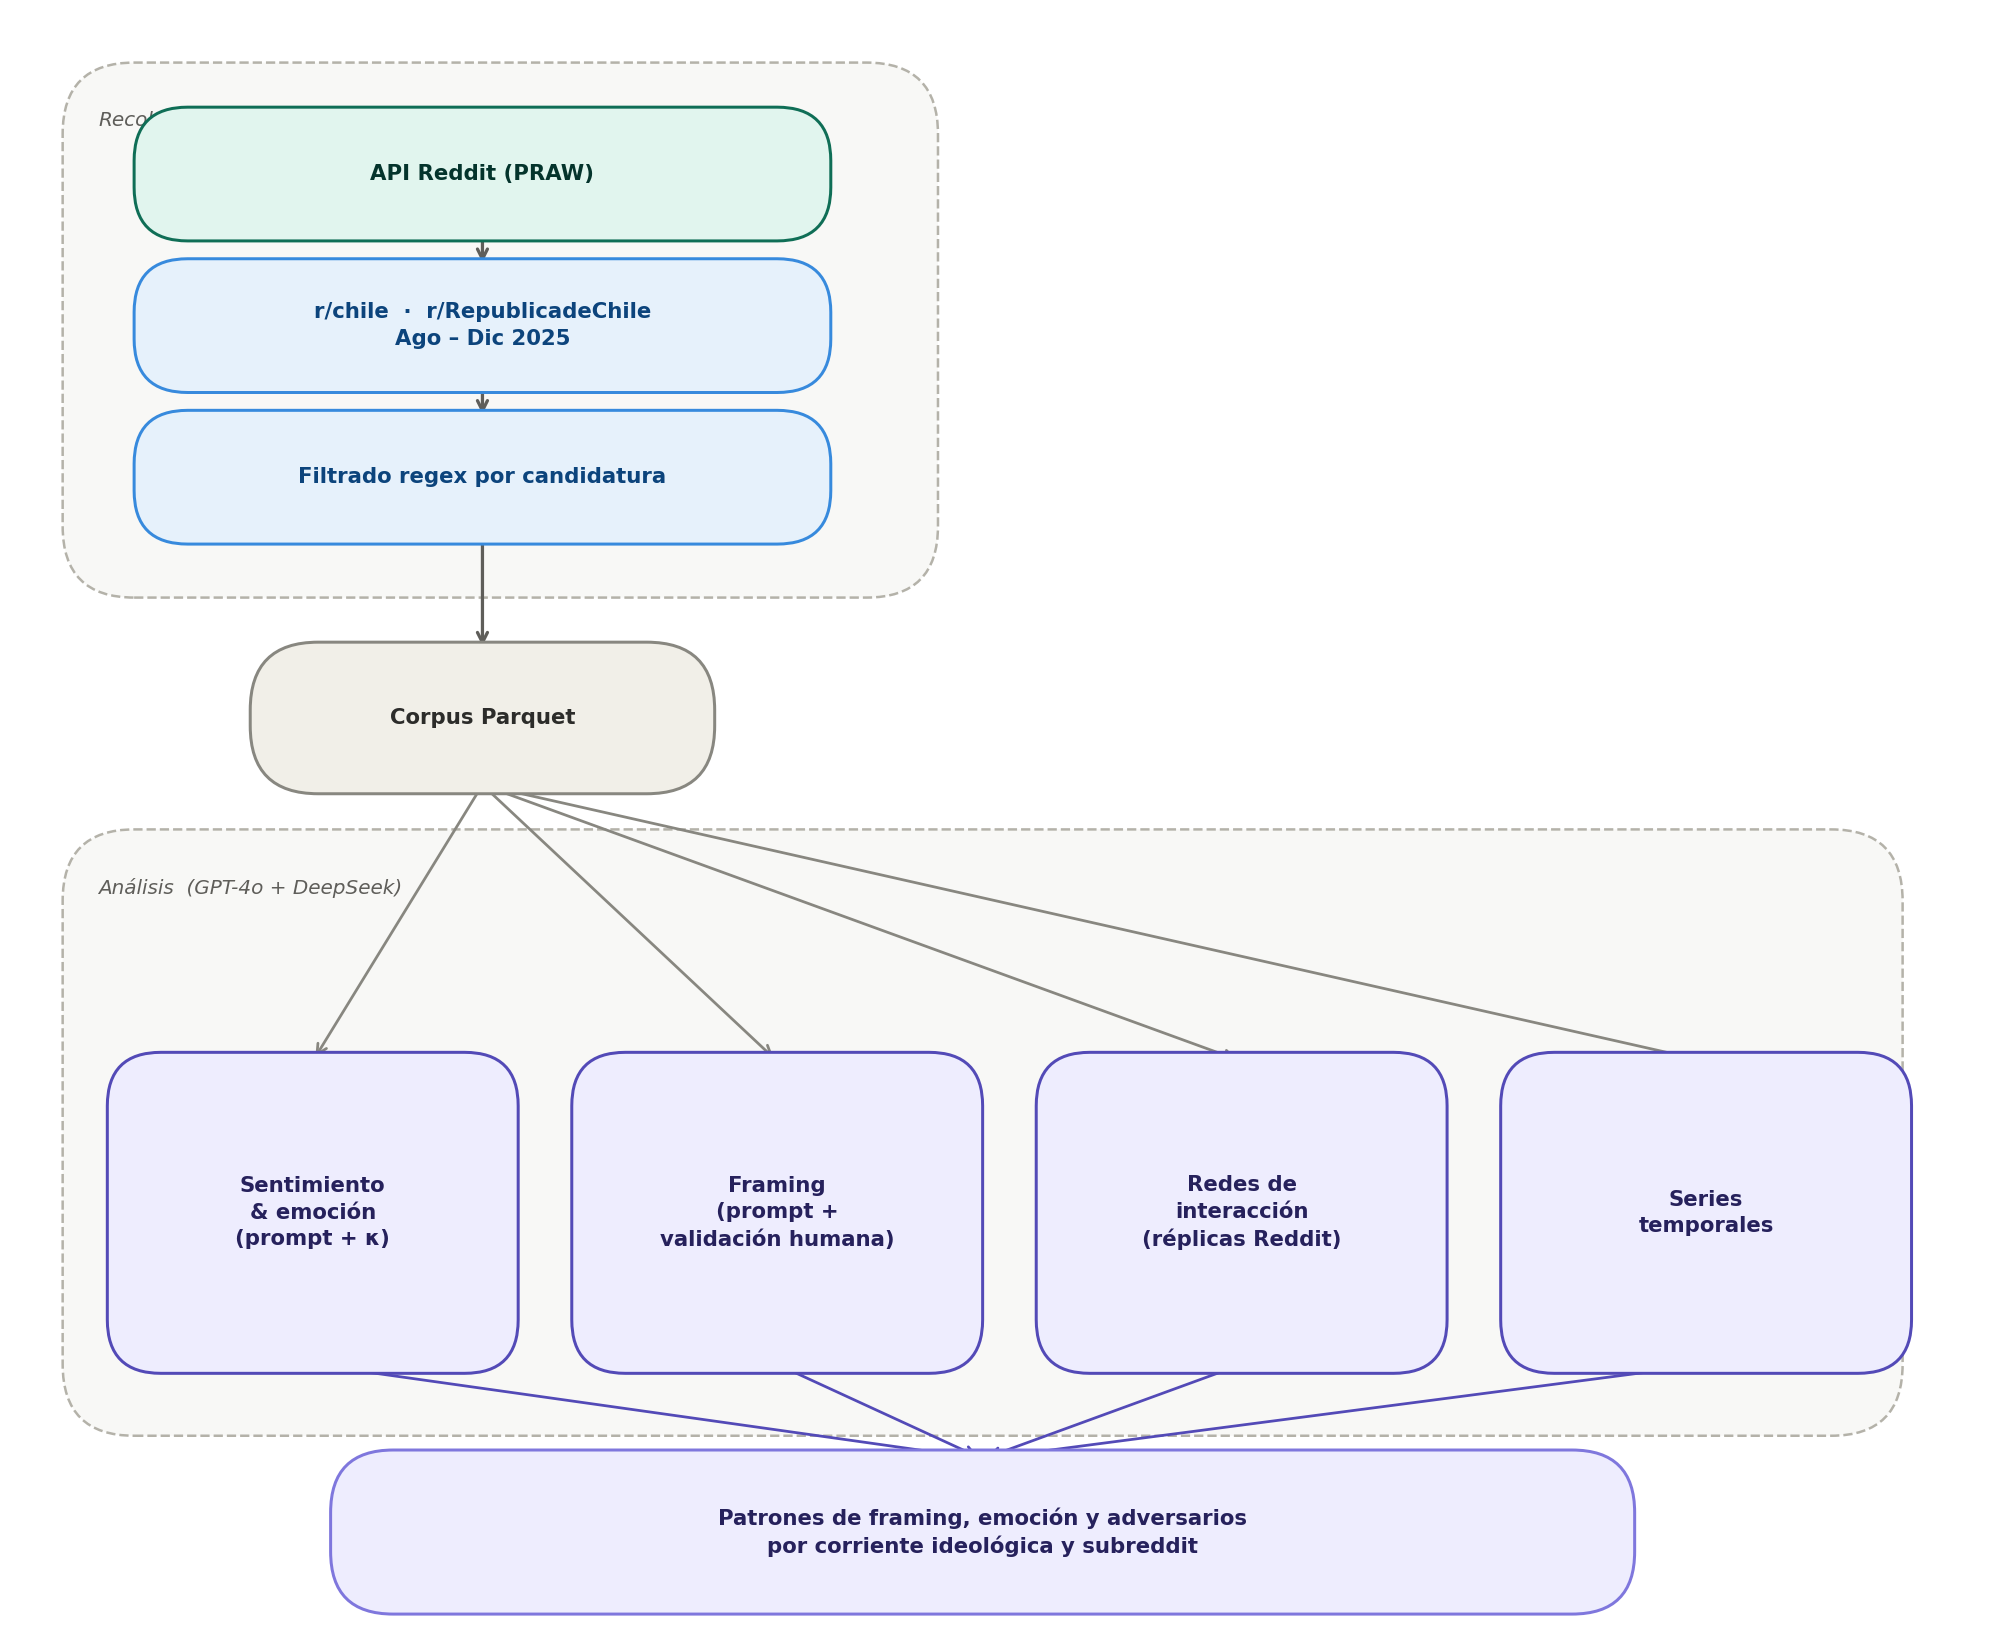
\includegraphics[width=0.9\textwidth,height=\textheight]{images/pipeline_corpus.png}

}

\caption{\label{fig-pipeline-datos}Flujo de recolección y procesamiento
del corpus.}

\end{figure}%

\bookmarksetup{startatroot}

\chapter{Depuración de Datos}\label{depuraciuxf3n-de-datos}

\bookmarksetup{startatroot}

\chapter{Exploración de Datos}\label{exploraciuxf3n-de-datos}

\bookmarksetup{startatroot}

\chapter{Modelado de Datos}\label{modelado-de-datos}

{[}Contenido de modelado de datos{]}

\section{Clustering K-Means}\label{clustering-k-means}

{[}Contenido sobre clustering K-Means{]}

\section{Clustering DBSCAN}\label{clustering-dbscan}

{[}Contenido sobre clustering DBSCAN{]}

\section{Clustering Jerárquico}\label{clustering-jeruxe1rquico}

{[}Contenido sobre clustering jerárquico{]}

\section{Determinación del modelo más
óptimo}\label{determinaciuxf3n-del-modelo-muxe1s-uxf3ptimo}

{[}Contenido sobre determinación del modelo más óptimo{]}

\bookmarksetup{startatroot}

\chapter{Interpretación de
Resultados}\label{interpretaciuxf3n-de-resultados}

{[}Contenido de interpretación de resultados{]}

\section{Interpretación de componentes
principales}\label{interpretaciuxf3n-de-componentes-principales}

{[}Contenido sobre interpretación de componentes principales{]}

\section{Interpretación de
clusters}\label{interpretaciuxf3n-de-clusters}

{[}Contenido sobre interpretación de clusters{]}

\section{Validación de los
resultados}\label{validaciuxf3n-de-los-resultados}

{[}Contenido sobre validación de resultados{]}

\bookmarksetup{startatroot}

\chapter{Conclusión}\label{conclusiuxf3n}

{[}Contenido de la conclusión{]}

\bookmarksetup{startatroot}

\chapter{Referencias}\label{referencias}

\phantomsection\label{refs}
\begin{CSLReferences}{0}{1}
\end{CSLReferences}




\end{document}
